\documentclass[]{article}
\usepackage{lmodern}
\usepackage{amssymb,amsmath}
\usepackage{ifxetex,ifluatex}
\usepackage{fixltx2e} % provides \textsubscript
\ifnum 0\ifxetex 1\fi\ifluatex 1\fi=0 % if pdftex
  \usepackage[T1]{fontenc}
  \usepackage[utf8]{inputenc}
\else % if luatex or xelatex
  \ifxetex
    \usepackage{mathspec}
  \else
    \usepackage{fontspec}
  \fi
  \defaultfontfeatures{Ligatures=TeX,Scale=MatchLowercase}
\fi
% use upquote if available, for straight quotes in verbatim environments
\IfFileExists{upquote.sty}{\usepackage{upquote}}{}
% use microtype if available
\IfFileExists{microtype.sty}{%
\usepackage{microtype}
\UseMicrotypeSet[protrusion]{basicmath} % disable protrusion for tt fonts
}{}
\usepackage[margin=1in]{geometry}
\usepackage{hyperref}
\hypersetup{unicode=true,
            pdftitle={710 Lab 10},
            pdfauthor={Talia Neal},
            pdfborder={0 0 0},
            breaklinks=true}
\urlstyle{same}  % don't use monospace font for urls
\usepackage{color}
\usepackage{fancyvrb}
\newcommand{\VerbBar}{|}
\newcommand{\VERB}{\Verb[commandchars=\\\{\}]}
\DefineVerbatimEnvironment{Highlighting}{Verbatim}{commandchars=\\\{\}}
% Add ',fontsize=\small' for more characters per line
\usepackage{framed}
\definecolor{shadecolor}{RGB}{248,248,248}
\newenvironment{Shaded}{\begin{snugshade}}{\end{snugshade}}
\newcommand{\KeywordTok}[1]{\textcolor[rgb]{0.13,0.29,0.53}{\textbf{#1}}}
\newcommand{\DataTypeTok}[1]{\textcolor[rgb]{0.13,0.29,0.53}{#1}}
\newcommand{\DecValTok}[1]{\textcolor[rgb]{0.00,0.00,0.81}{#1}}
\newcommand{\BaseNTok}[1]{\textcolor[rgb]{0.00,0.00,0.81}{#1}}
\newcommand{\FloatTok}[1]{\textcolor[rgb]{0.00,0.00,0.81}{#1}}
\newcommand{\ConstantTok}[1]{\textcolor[rgb]{0.00,0.00,0.00}{#1}}
\newcommand{\CharTok}[1]{\textcolor[rgb]{0.31,0.60,0.02}{#1}}
\newcommand{\SpecialCharTok}[1]{\textcolor[rgb]{0.00,0.00,0.00}{#1}}
\newcommand{\StringTok}[1]{\textcolor[rgb]{0.31,0.60,0.02}{#1}}
\newcommand{\VerbatimStringTok}[1]{\textcolor[rgb]{0.31,0.60,0.02}{#1}}
\newcommand{\SpecialStringTok}[1]{\textcolor[rgb]{0.31,0.60,0.02}{#1}}
\newcommand{\ImportTok}[1]{#1}
\newcommand{\CommentTok}[1]{\textcolor[rgb]{0.56,0.35,0.01}{\textit{#1}}}
\newcommand{\DocumentationTok}[1]{\textcolor[rgb]{0.56,0.35,0.01}{\textbf{\textit{#1}}}}
\newcommand{\AnnotationTok}[1]{\textcolor[rgb]{0.56,0.35,0.01}{\textbf{\textit{#1}}}}
\newcommand{\CommentVarTok}[1]{\textcolor[rgb]{0.56,0.35,0.01}{\textbf{\textit{#1}}}}
\newcommand{\OtherTok}[1]{\textcolor[rgb]{0.56,0.35,0.01}{#1}}
\newcommand{\FunctionTok}[1]{\textcolor[rgb]{0.00,0.00,0.00}{#1}}
\newcommand{\VariableTok}[1]{\textcolor[rgb]{0.00,0.00,0.00}{#1}}
\newcommand{\ControlFlowTok}[1]{\textcolor[rgb]{0.13,0.29,0.53}{\textbf{#1}}}
\newcommand{\OperatorTok}[1]{\textcolor[rgb]{0.81,0.36,0.00}{\textbf{#1}}}
\newcommand{\BuiltInTok}[1]{#1}
\newcommand{\ExtensionTok}[1]{#1}
\newcommand{\PreprocessorTok}[1]{\textcolor[rgb]{0.56,0.35,0.01}{\textit{#1}}}
\newcommand{\AttributeTok}[1]{\textcolor[rgb]{0.77,0.63,0.00}{#1}}
\newcommand{\RegionMarkerTok}[1]{#1}
\newcommand{\InformationTok}[1]{\textcolor[rgb]{0.56,0.35,0.01}{\textbf{\textit{#1}}}}
\newcommand{\WarningTok}[1]{\textcolor[rgb]{0.56,0.35,0.01}{\textbf{\textit{#1}}}}
\newcommand{\AlertTok}[1]{\textcolor[rgb]{0.94,0.16,0.16}{#1}}
\newcommand{\ErrorTok}[1]{\textcolor[rgb]{0.64,0.00,0.00}{\textbf{#1}}}
\newcommand{\NormalTok}[1]{#1}
\usepackage{graphicx,grffile}
\makeatletter
\def\maxwidth{\ifdim\Gin@nat@width>\linewidth\linewidth\else\Gin@nat@width\fi}
\def\maxheight{\ifdim\Gin@nat@height>\textheight\textheight\else\Gin@nat@height\fi}
\makeatother
% Scale images if necessary, so that they will not overflow the page
% margins by default, and it is still possible to overwrite the defaults
% using explicit options in \includegraphics[width, height, ...]{}
\setkeys{Gin}{width=\maxwidth,height=\maxheight,keepaspectratio}
\IfFileExists{parskip.sty}{%
\usepackage{parskip}
}{% else
\setlength{\parindent}{0pt}
\setlength{\parskip}{6pt plus 2pt minus 1pt}
}
\setlength{\emergencystretch}{3em}  % prevent overfull lines
\providecommand{\tightlist}{%
  \setlength{\itemsep}{0pt}\setlength{\parskip}{0pt}}
\setcounter{secnumdepth}{0}
% Redefines (sub)paragraphs to behave more like sections
\ifx\paragraph\undefined\else
\let\oldparagraph\paragraph
\renewcommand{\paragraph}[1]{\oldparagraph{#1}\mbox{}}
\fi
\ifx\subparagraph\undefined\else
\let\oldsubparagraph\subparagraph
\renewcommand{\subparagraph}[1]{\oldsubparagraph{#1}\mbox{}}
\fi

%%% Use protect on footnotes to avoid problems with footnotes in titles
\let\rmarkdownfootnote\footnote%
\def\footnote{\protect\rmarkdownfootnote}

%%% Change title format to be more compact
\usepackage{titling}

% Create subtitle command for use in maketitle
\newcommand{\subtitle}[1]{
  \posttitle{
    \begin{center}\large#1\end{center}
    }
}

\setlength{\droptitle}{-2em}
  \title{710 Lab 10}
  \pretitle{\vspace{\droptitle}\centering\huge}
  \posttitle{\par}
\subtitle{multiple regression}
  \author{Talia Neal}
  \preauthor{\centering\large\emph}
  \postauthor{\par}
  \predate{\centering\large\emph}
  \postdate{\par}
  \date{11.7.18}


\begin{document}
\maketitle

\subsection{Problem 1}\label{problem-1}

\paragraph{Introduction:}\label{introduction}

The goal of this study is to determine which factors contribute most to
variance in tree plot biomass. To investigate which factors are most
useful in predicting biomass of trees, information on tree height, wood
density, basal area, wood diameter, and trees falls (broken down by tree
size) were collected and analyzed with multiple linear regression
modeling.. The null hypothesis for the saturated model is that there is
no signficant relationship of plot biomass to any of the above
variables. The alternative hypothis is that there is a signficant linear
relationship between plot biomass and at least one of the 5
variables/interactions. After examination of the results obtained from
the saturated model, parameters appearing to be less significant were
considered for removal in order to obtain the minimum adequate model.
For each of these tests, the null hypothesis is that the minimum model
is adequate and the alternative hypothesis is that it is not adequate.

\paragraph{Methods:}\label{methods}

The 70 tree plots include the variables: (1) plot biomass
(AGBH.Mg.ha),(2) mean tree diameter (mDBH.cm),(3) mean height (mH.m),
(4) mean wood density (mWD.g.m3), (5) mean basal area (mBA.cm2), and (6)
tree falls in the plot (Tree.Fall). All variables except for tree fall
are continuous data measurements of trees. Tree falls is a categorical
data set broken down into the following: minor, major and rien (large
tree, moderate sized tree, no tree fall).

As a first step, biomass was plotted vs tree diameter, tree height, wood
density, basal area, and tree falls. Based on these plots, all of these
factors appear to have a potential effect on biomass. A correlation test
showed that tree diameter, tree height, and basal area had a strong
correlation. Wood density showed a weaker correlation, but not
sufficiently low as to exclude it from an initial model. Based on the
boxplot of tree falls, it appears that major falls may positively impact
plot biomass, which all other fall types have approximately the same
effect. This will also be included in the model. A histogram of plot
biomass shows that the data is skewed towards lower values. The data
were log transformed and re-examined; they appeared to be farther from
normal than before and as such the original data will be used in the
model. After running the initial saturated model, factors which did not
appear to significantly affect biomass were removed one at a time,
checking each time to ensure that removal did not substantially reduce
the predictive capacity of the model.

\paragraph{Results:}\label{results}

The results of the saturated model indicated that tree falls and tree
height did not appear to be statistically significant (p \textgreater{}
.05). As such, the model was first updated to remove falls. This changed
the multiple r squared very little (from .5598 to .542), indicating that
this was a valid removal. The model was next updated to remove tree
height. This changed the multiple r squared from .542 to .533,
indicating once again that this was a valid removal. Finally, the model
wa updated to remove tree diameter as it also appeared to be
insignificant. This removal changed the multiple r squared from .533 to
.5328, indicating once again that this was a valid removal. Though tree
basal area, and wood density do appear to be significant, additional
models were run with these parameters removed to verify their
significance. Removal of area and density reduced the multiple r squared
by \textasciitilde{}.2 and \textasciitilde{}.1 respectively, indicating
that significantly less variance was explained with the removal of
either parameter. Therefore, a reduced model with only basal area and
wood density appears to be the minimum adequate model. The diagnostics
for this model indicate that the data appear fairly normal and
homoscedacity is appropriate. However, there are a couple of points (47
\& 50) that do appear to have a good deal of leverage based on the Cooks
distance. If these were my actual data I would reexamine those data
points. As a final check, collinearity between these two parameters was
checked with the variance inflation factor (VIF) and found to be 1.18,
indicating a low level of collinearity between the factors.

Therefore, the minimum adequate model was found to be: Biomass = -286.67
+ 587.6(Density) + .313(Basal Area) Both wood density and basal area
positively impact plot biomass, and all other parameters were found to
be insignificant. P values for both factors were well below .05,
indicating that they are both highly significant. The multiple r squared
for this model is .53, indicating that these two parameters explain
around half of the variance in tree plot biomass observed.

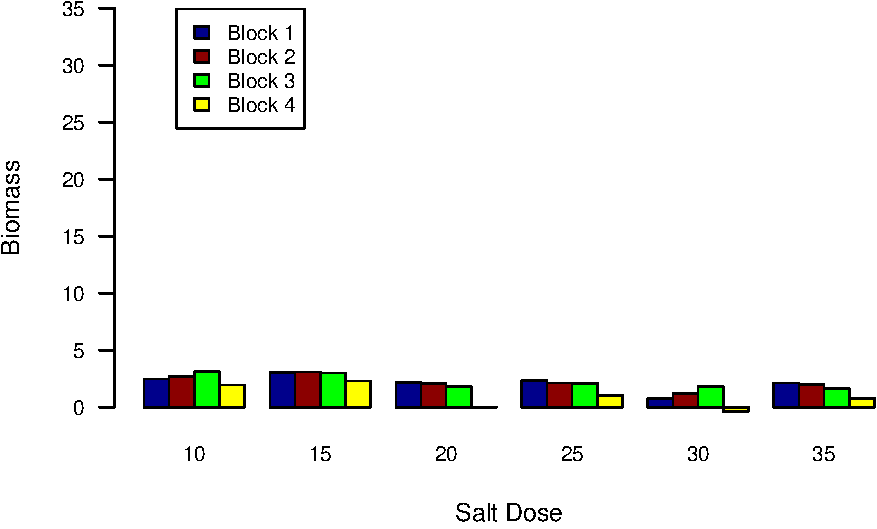
\includegraphics{710_lab_10_files/figure-latex/unnamed-chunk-1-1.pdf}

\begin{verbatim}
## 
##  Pearson's product-moment correlation
## 
## data:  diameter and biomass
## t = 7.2096, df = 68, p-value = 5.94e-10
## alternative hypothesis: true correlation is not equal to 0
## 95 percent confidence interval:
##  0.5006601 0.7735399
## sample estimates:
##       cor 
## 0.6582019
\end{verbatim}

\begin{verbatim}
## 
##  Pearson's product-moment correlation
## 
## data:  height and biomass
## t = 6.6606, df = 68, p-value = 5.767e-09
## alternative hypothesis: true correlation is not equal to 0
## 95 percent confidence interval:
##  0.4615114 0.7522533
## sample estimates:
##       cor 
## 0.6283456
\end{verbatim}

\begin{verbatim}
## 
##  Pearson's product-moment correlation
## 
## data:  density and biomass
## t = 5.4856, df = 68, p-value = 6.567e-07
## alternative hypothesis: true correlation is not equal to 0
## 95 percent confidence interval:
##  0.3666100 0.6980035
## sample estimates:
##       cor 
## 0.5538714
\end{verbatim}

\begin{verbatim}
## 
##  Pearson's product-moment correlation
## 
## data:  area and biomass
## t = 7.1542, df = 68, p-value = 7.479e-10
## alternative hypothesis: true correlation is not equal to 0
## 95 percent confidence interval:
##  0.4968536 0.7714969
## sample estimates:
##       cor 
## 0.6553205
\end{verbatim}

\includegraphics{710_lab_10_files/figure-latex/unnamed-chunk-2-1.pdf}

\begin{verbatim}
## 
## Call:
## lm(formula = biomass ~ diameter + height + density + area + factor(falls))
## 
## Residuals:
##     Min      1Q  Median      3Q     Max 
## -278.30  -42.78   13.42   40.80  235.97 
## 
## Coefficients:
##                      Estimate Std. Error t value Pr(>|t|)    
## (Intercept)         -423.8723   173.2292  -2.447 0.017258 *  
## diameter             -72.9733    70.1023  -1.041 0.301939    
## height                91.9557    81.5644   1.127 0.263918    
## density              624.5868   169.1739   3.692 0.000472 ***
## area                   0.7226     0.4976   1.452 0.151472    
## factor(falls)majeur   40.9792    43.1042   0.951 0.345448    
## factor(falls)mineur   -2.9520    38.0787  -0.078 0.938456    
## factor(falls)rien     -5.2892    40.1616  -0.132 0.895649    
## ---
## Signif. codes:  0 '***' 0.001 '**' 0.01 '*' 0.05 '.' 0.1 ' ' 1
## 
## Residual standard error: 87.29 on 62 degrees of freedom
## Multiple R-squared:  0.5598, Adjusted R-squared:  0.5101 
## F-statistic: 11.26 on 7 and 62 DF,  p-value: 4.133e-09
\end{verbatim}

\begin{verbatim}
## 
## Call:
## lm(formula = biomass ~ diameter + height + density + area)
## 
## Residuals:
##     Min      1Q  Median      3Q     Max 
## -288.35  -45.81   13.20   52.17  221.90 
## 
## Coefficients:
##              Estimate Std. Error t value Pr(>|t|)    
## (Intercept) -367.9127   157.4008  -2.337 0.022508 *  
## diameter     -75.9287    69.0505  -1.100 0.275558    
## height        91.2898    80.4782   1.134 0.260817    
## density      585.2154   162.0312   3.612 0.000593 ***
## area           0.8080     0.4844   1.668 0.100113    
## ---
## Signif. codes:  0 '***' 0.001 '**' 0.01 '*' 0.05 '.' 0.1 ' ' 1
## 
## Residual standard error: 86.95 on 65 degrees of freedom
## Multiple R-squared:  0.542,  Adjusted R-squared:  0.5139 
## F-statistic: 19.23 on 4 and 65 DF,  p-value: 1.765e-10
\end{verbatim}

\begin{verbatim}
## 
## Call:
## lm(formula = biomass ~ diameter + density + area)
## 
## Residuals:
##     Min      1Q  Median      3Q     Max 
## -300.56  -31.89   12.15   47.56  233.84 
## 
## Coefficients:
##              Estimate Std. Error t value Pr(>|t|)    
## (Intercept) -302.9337   146.9252  -2.062 0.043166 *  
## diameter       1.4625    10.6642   0.137 0.891338    
## density      580.4436   162.3281   3.576 0.000659 ***
## area           0.2914     0.1653   1.763 0.082572 .  
## ---
## Signif. codes:  0 '***' 0.001 '**' 0.01 '*' 0.05 '.' 0.1 ' ' 1
## 
## Residual standard error: 87.14 on 66 degrees of freedom
## Multiple R-squared:  0.533,  Adjusted R-squared:  0.5118 
## F-statistic: 25.11 on 3 and 66 DF,  p-value: 5.937e-11
\end{verbatim}

\begin{verbatim}
## 
## Call:
## lm(formula = biomass ~ density + area)
## 
## Residuals:
##     Min      1Q  Median      3Q     Max 
## -304.74  -30.83   11.75   46.51  233.10 
## 
## Coefficients:
##               Estimate Std. Error t value Pr(>|t|)    
## (Intercept) -286.67527   86.14930  -3.328 0.001425 ** 
## density      587.59879  152.58513   3.851 0.000266 ***
## area           0.31271    0.05492   5.694 2.99e-07 ***
## ---
## Signif. codes:  0 '***' 0.001 '**' 0.01 '*' 0.05 '.' 0.1 ' ' 1
## 
## Residual standard error: 86.5 on 67 degrees of freedom
## Multiple R-squared:  0.5328, Adjusted R-squared:  0.5189 
## F-statistic: 38.21 on 2 and 67 DF,  p-value: 8.451e-12
\end{verbatim}

\includegraphics{710_lab_10_files/figure-latex/unnamed-chunk-3-1.pdf}

\begin{verbatim}
## Loading required package: carData
\end{verbatim}

\begin{verbatim}
## 
## Attaching package: 'car'
\end{verbatim}

\begin{verbatim}
## The following object is masked from 'package:openintro':
## 
##     densityPlot
\end{verbatim}

\begin{verbatim}
##  density     area 
## 1.184032 1.184032
\end{verbatim}

\includegraphics{710_lab_10_files/figure-latex/unnamed-chunk-4-1.pdf}
\includegraphics{710_lab_10_files/figure-latex/unnamed-chunk-5-1.pdf}

\subsection{Problem 2}\label{problem-2}

\paragraph{Introduction}\label{introduction-1}

The goal of this study is to determine which factors contribute most to
variance in atmospheric ozone concentration. To investigate which
factors are most useful in predicting ozone concentration, measurements
for temperature, solar radiation, and wind speed were collected and
analyzed with multiple linear regression modeling. The null hypothesis
for the saturated model is that there is no signficant relationship of
ozone concentration to any of the above variables or their interactions.
The alternative hypothis is that there is a signficant linear
relationship between ozone concentration and at least one of the 3
variables/interactions. After examination of the results obtained from
the saturated model, parameters appearing to be less significant were
considered for removal in order to obtain the minimum adequate model.
For each of these tests, the null hypothesis is that the minimum model
is adequate and the alternative hypothesis is that it is not adequate.

\paragraph{Methods:}\label{methods-1}

These data include the variables: (1) ozone (ozone),(2) solar radiation
(rad),(3) temperature (temp), and (4) wind speed wind., All variables
are continuous data measurements.

As a first step, ozone was plotted vs.~radiation, temperature, and wind.
Based on these plots, wind and temperature show a clear corellation.
However, it is unclear if radiation is corellated. A corellation test
indicated a corellation of \textasciitilde{}.6 for wind and temperate,
and \textasciitilde{}.3 for radiation. As such, all factors and their
potential interactions were included in the saturated model. A histogram
of ozone concentration shows that the data is heavily skewed towards
lower values. The data were log transformed and re-examined; they
appeared to be much closer to a normal distribution than before.
Therefore, log transformed ozone concentration data will be used in the
model. After running the initial saturated model, factors which did not
appear to significantly affect biomass were removed one at a time,
checking each time to ensure that removal did not substantially reduce
the predictive capacity of the model.

\paragraph{Results:}\label{results-1}

The results of the saturated model indicated that none of the
interaction terms were significant. They were removed one at a time in
order of highest to lowest p value. Removal of radiaiton-temperature
interaction resulted in no change in multiple r squared. Removal of the
radiation-wind interaction changed the multiple r squared value from
.6801 to .679. Removal of the temperature-wind interaction changed the
multiple r squared from .679 to .6649. These very small changes indicate
that none of the interaction terms are needed in the minimum adequate
model. The model with all interaction terms removed indicated that all
remaining factors were significant. As a last check, radiation, wind
speed, and temperature were all independantly removed to verify that
removal of the parameter would significantly impact the model. The
removal of wind or radiation decreased the multiple r squared by
\textasciitilde{}.05 and \textasciitilde{}.1, respectively; removing
temperature decreased the multiple r squared by \textasciitilde{}.2. I
therefore chose to remove wind and include only radiation and
temperature in the minimally adequate model. The diagnostics for this
model indicate that the data appear fairly normal. The residual plots
may have some unaccounted for structure, but not so much as to be
unacceptable. Point 17 does appear to potentially be a bit of an outlier
based on the Cooks distance and could therefore use a verification. As a
final check, collinearity between these two parameters was checked with
the variance inflation factor (VIF) and found to be 1.09, indicating a
low level of collinearity between the factors in the reduced model.

Therefore, the minimum adequate model was found to be: ozone = -1.76 +
.0025(radiation) + .0607(temperature) However, this model is in log
units, for ease of use, it may be converted to original scale. This
results in the model: ozone = .017 + 1.002(radiation) +
1.06(temperature) P values for this model were both well below .05,
indicating that these two parameters are highly significant. The
multiple r squared for the reduced model is .616, indicating that these
two parameters explain roughly 60\% of variance in atmospheric ozone
concentration.

\begin{Shaded}
\begin{Highlighting}[]
\NormalTok{dat <-}\StringTok{ }\KeywordTok{read.csv}\NormalTok{(}\StringTok{"ozone.data.csv"}\NormalTok{)}
\NormalTok{ozone <-}\StringTok{ }\NormalTok{dat}\OperatorTok{$}\NormalTok{ozone}
\NormalTok{rad <-}\StringTok{ }\NormalTok{dat}\OperatorTok{$}\NormalTok{rad}
\NormalTok{temp <-}\StringTok{ }\NormalTok{dat}\OperatorTok{$}\NormalTok{temp}
\NormalTok{wind <-}\StringTok{ }\NormalTok{dat}\OperatorTok{$}\NormalTok{wind}
\KeywordTok{par}\NormalTok{(}\DataTypeTok{mfrow =} \KeywordTok{c}\NormalTok{(}\DecValTok{2}\NormalTok{,}\DecValTok{2}\NormalTok{))}
\KeywordTok{plot}\NormalTok{(rad, ozone)}
\KeywordTok{plot}\NormalTok{(wind, ozone)}
\KeywordTok{plot}\NormalTok{(temp, ozone)}
\KeywordTok{cor.test}\NormalTok{(rad, ozone)}
\end{Highlighting}
\end{Shaded}

\begin{verbatim}
## 
##  Pearson's product-moment correlation
## 
## data:  rad and ozone
## t = 3.8798, df = 109, p-value = 0.0001793
## alternative hypothesis: true correlation is not equal to 0
## 95 percent confidence interval:
##  0.173194 0.502132
## sample estimates:
##       cor 
## 0.3483417
\end{verbatim}

\begin{Shaded}
\begin{Highlighting}[]
\KeywordTok{cor.test}\NormalTok{(temp, ozone)}
\end{Highlighting}
\end{Shaded}

\begin{verbatim}
## 
##  Pearson's product-moment correlation
## 
## data:  temp and ozone
## t = 10.192, df = 109, p-value < 2.2e-16
## alternative hypothesis: true correlation is not equal to 0
## 95 percent confidence interval:
##  0.5888139 0.7829869
## sample estimates:
##       cor 
## 0.6985414
\end{verbatim}

\begin{Shaded}
\begin{Highlighting}[]
\KeywordTok{cor.test}\NormalTok{(wind, ozone)}
\end{Highlighting}
\end{Shaded}

\begin{verbatim}
## 
##  Pearson's product-moment correlation
## 
## data:  wind and ozone
## t = -8.0993, df = 109, p-value = 8.652e-13
## alternative hypothesis: true correlation is not equal to 0
## 95 percent confidence interval:
##  -0.7173829 -0.4815780
## sample estimates:
##        cor 
## -0.6129508
\end{verbatim}

\begin{Shaded}
\begin{Highlighting}[]
\KeywordTok{par}\NormalTok{(}\DataTypeTok{mfrow =} \KeywordTok{c}\NormalTok{(}\DecValTok{1}\NormalTok{,}\DecValTok{2}\NormalTok{))}
\end{Highlighting}
\end{Shaded}

\includegraphics{710_lab_10_files/figure-latex/unnamed-chunk-6-1.pdf}

\begin{Shaded}
\begin{Highlighting}[]
\KeywordTok{hist}\NormalTok{(ozone)}
\KeywordTok{hist}\NormalTok{(}\KeywordTok{log}\NormalTok{(ozone))}
\end{Highlighting}
\end{Shaded}

\includegraphics{710_lab_10_files/figure-latex/unnamed-chunk-6-2.pdf}

\begin{Shaded}
\begin{Highlighting}[]
\NormalTok{lm00 <-}\StringTok{ }\KeywordTok{with}\NormalTok{(dat, }\KeywordTok{lm}\NormalTok{(}\KeywordTok{log}\NormalTok{(ozone) }\OperatorTok{~}\StringTok{ }\NormalTok{rad }\OperatorTok{+}\StringTok{ }\NormalTok{temp }\OperatorTok{+}\StringTok{ }\NormalTok{wind }\OperatorTok{+}\StringTok{ }\NormalTok{rad}\OperatorTok{:}\NormalTok{temp }\OperatorTok{+}\StringTok{ }\NormalTok{rad}\OperatorTok{:}\NormalTok{wind }\OperatorTok{+}\StringTok{ }\NormalTok{temp}\OperatorTok{:}\NormalTok{wind))}
\KeywordTok{summary}\NormalTok{(lm00)}
\end{Highlighting}
\end{Shaded}

\begin{verbatim}
## 
## Call:
## lm(formula = log(ozone) ~ rad + temp + wind + rad:temp + rad:wind + 
##     temp:wind)
## 
## Residuals:
##      Min       1Q   Median       3Q      Max 
## -1.98599 -0.34242 -0.04091  0.31039  1.18626 
## 
## Coefficients:
##               Estimate Std. Error t value Pr(>|t|)   
## (Intercept) -2.351e+00  1.687e+00  -1.394  0.16639   
## rad          3.173e-03  5.536e-03   0.573  0.56773   
## temp         7.266e-02  2.189e-02   3.319  0.00124 **
## wind         1.497e-01  1.127e-01   1.328  0.18704   
## rad:temp     6.393e-06  6.424e-05   0.100  0.92092   
## rad:wind    -9.593e-05  1.757e-04  -0.546  0.58624   
## temp:wind   -2.487e-03  1.549e-03  -1.605  0.11146   
## ---
## Signif. codes:  0 '***' 0.001 '**' 0.01 '*' 0.05 '.' 0.1 ' ' 1
## 
## Residual standard error: 0.5037 on 104 degrees of freedom
## Multiple R-squared:  0.6801, Adjusted R-squared:  0.6616 
## F-statistic: 36.85 on 6 and 104 DF,  p-value: < 2.2e-16
\end{verbatim}

\begin{Shaded}
\begin{Highlighting}[]
\CommentTok{#Based on the saturated model, rad:wind is definitely not important. Let's take it out. }
\NormalTok{lm11 <-}\StringTok{ }\KeywordTok{update}\NormalTok{(lm00, }\OperatorTok{~}\NormalTok{.}\OperatorTok{-}\NormalTok{rad}\OperatorTok{:}\NormalTok{temp)}
\KeywordTok{summary}\NormalTok{(lm11)}
\end{Highlighting}
\end{Shaded}

\begin{verbatim}
## 
## Call:
## lm(formula = log(ozone) ~ rad + temp + wind + rad:wind + temp:wind)
## 
## Residuals:
##     Min      1Q  Median      3Q     Max 
## -1.9699 -0.3408 -0.0401  0.3095  1.1910 
## 
## Coefficients:
##               Estimate Std. Error t value Pr(>|t|)    
## (Intercept) -2.4669097  1.2136987  -2.033   0.0446 *  
## rad          0.0036894  0.0019308   1.911   0.0588 .  
## temp         0.0741154  0.0161944   4.577  1.3e-05 ***
## wind         0.1527897  0.1080035   1.415   0.1601    
## rad:wind    -0.0001003  0.0001694  -0.592   0.5552    
## temp:wind   -0.0025158  0.0015152  -1.660   0.0998 .  
## ---
## Signif. codes:  0 '***' 0.001 '**' 0.01 '*' 0.05 '.' 0.1 ' ' 1
## 
## Residual standard error: 0.5013 on 105 degrees of freedom
## Multiple R-squared:  0.6801, Adjusted R-squared:  0.6648 
## F-statistic: 44.64 on 5 and 105 DF,  p-value: < 2.2e-16
\end{verbatim}

\begin{Shaded}
\begin{Highlighting}[]
\NormalTok{lm12 <-}\StringTok{ }\KeywordTok{update}\NormalTok{(lm11, }\OperatorTok{~}\NormalTok{.}\OperatorTok{-}\NormalTok{rad}\OperatorTok{:}\NormalTok{wind)}
\KeywordTok{summary}\NormalTok{(lm12)}
\end{Highlighting}
\end{Shaded}

\begin{verbatim}
## 
## Call:
## lm(formula = log(ozone) ~ rad + temp + wind + temp:wind)
## 
## Residuals:
##      Min       1Q   Median       3Q      Max 
## -1.98696 -0.32076 -0.05428  0.30238  1.19016 
## 
## Coefficients:
##               Estimate Std. Error t value Pr(>|t|)    
## (Intercept) -2.5845520  1.1936395  -2.165   0.0326 *  
## rad          0.0025939  0.0005483   4.731 6.93e-06 ***
## temp         0.0782341  0.0145784   5.366 4.76e-07 ***
## wind         0.1661571  0.1052917   1.578   0.1175    
## temp:wind   -0.0029299  0.0013399  -2.187   0.0310 *  
## ---
## Signif. codes:  0 '***' 0.001 '**' 0.01 '*' 0.05 '.' 0.1 ' ' 1
## 
## Residual standard error: 0.4997 on 106 degrees of freedom
## Multiple R-squared:  0.679,  Adjusted R-squared:  0.6669 
## F-statistic: 56.05 on 4 and 106 DF,  p-value: < 2.2e-16
\end{verbatim}

\begin{Shaded}
\begin{Highlighting}[]
\NormalTok{lm13 <-}\StringTok{ }\KeywordTok{update}\NormalTok{(lm12, }\OperatorTok{~}\NormalTok{.}\OperatorTok{-}\NormalTok{temp}\OperatorTok{:}\NormalTok{wind)}
\KeywordTok{summary}\NormalTok{(lm13)}
\end{Highlighting}
\end{Shaded}

\begin{verbatim}
## 
## Call:
## lm(formula = log(ozone) ~ rad + temp + wind)
## 
## Residuals:
##      Min       1Q   Median       3Q      Max 
## -2.06212 -0.29968 -0.00223  0.30767  1.23572 
## 
## Coefficients:
##               Estimate Std. Error t value Pr(>|t|)    
## (Intercept) -0.2611739  0.5534102  -0.472 0.637934    
## rad          0.0025147  0.0005567   4.518 1.62e-05 ***
## temp         0.0491630  0.0060863   8.078 1.07e-12 ***
## wind        -0.0615925  0.0157037  -3.922 0.000155 ***
## ---
## Signif. codes:  0 '***' 0.001 '**' 0.01 '*' 0.05 '.' 0.1 ' ' 1
## 
## Residual standard error: 0.5085 on 107 degrees of freedom
## Multiple R-squared:  0.6645, Adjusted R-squared:  0.6551 
## F-statistic: 70.65 on 3 and 107 DF,  p-value: < 2.2e-16
\end{verbatim}

\begin{Shaded}
\begin{Highlighting}[]
\NormalTok{lm14<-}\StringTok{ }\KeywordTok{update}\NormalTok{(lm13, }\OperatorTok{~}\NormalTok{.}\OperatorTok{-}\NormalTok{wind)}
\KeywordTok{summary}\NormalTok{(lm14)}
\end{Highlighting}
\end{Shaded}

\begin{verbatim}
## 
## Call:
## lm(formula = log(ozone) ~ rad + temp)
## 
## Residuals:
##      Min       1Q   Median       3Q      Max 
## -1.83864 -0.33727  0.03444  0.29877  1.38210 
## 
## Coefficients:
##               Estimate Std. Error t value Pr(>|t|)    
## (Intercept) -1.7646527  0.4249016  -4.153 6.58e-05 ***
## rad          0.0024651  0.0005924   4.161 6.38e-05 ***
## temp         0.0607386  0.0056663  10.719  < 2e-16 ***
## ---
## Signif. codes:  0 '***' 0.001 '**' 0.01 '*' 0.05 '.' 0.1 ' ' 1
## 
## Residual standard error: 0.5413 on 108 degrees of freedom
## Multiple R-squared:  0.6163, Adjusted R-squared:  0.6092 
## F-statistic: 86.73 on 2 and 108 DF,  p-value: < 2.2e-16
\end{verbatim}

\begin{Shaded}
\begin{Highlighting}[]
\CommentTok{#lm15<- update(lm14, ~.-rad)}
\CommentTok{#summary(lm15)}
\CommentTok{#lm14 is the minimum adequate model. Let's look at diagnostics. }
  \KeywordTok{par}\NormalTok{(}\DataTypeTok{mfrow =} \KeywordTok{c}\NormalTok{(}\DecValTok{2}\NormalTok{,}\DecValTok{2}\NormalTok{)) }
  \KeywordTok{plot}\NormalTok{(lm14)}
\end{Highlighting}
\end{Shaded}

\includegraphics{710_lab_10_files/figure-latex/unnamed-chunk-7-1.pdf}

\begin{Shaded}
\begin{Highlighting}[]
 \CommentTok{#The variance inflation factor (VIF) is an index of how much the variance of an estimated regression coefficient increases because of collinearity. A common rule of thumb is that if VIF(βˆ) > 5, then multicollinearity is high}
\KeywordTok{library}\NormalTok{(car)}
\KeywordTok{vif}\NormalTok{(lm14)}
\end{Highlighting}
\end{Shaded}

\begin{verbatim}
##      rad     temp 
## 1.094676 1.094676
\end{verbatim}

\begin{verbatim}
## (Intercept)         rad        temp 
##   0.1712463   1.0024682   1.0626211
\end{verbatim}

\includegraphics{710_lab_10_files/figure-latex/unnamed-chunk-8-1.pdf}
\includegraphics{710_lab_10_files/figure-latex/unnamed-chunk-9-1.pdf}

\begin{Shaded}
\begin{Highlighting}[]
\NormalTok{plots <-}\StringTok{ }\KeywordTok{read.csv}\NormalTok{(}\StringTok{"TreePlots-2.csv"}\NormalTok{)}
\NormalTok{biomass <-plots}\OperatorTok{$}\NormalTok{AGBH.Mg.h}
\NormalTok{diameter <-}\StringTok{ }\NormalTok{plots}\OperatorTok{$}\NormalTok{mDBH.cm}
\NormalTok{height <-}\StringTok{ }\NormalTok{plots}\OperatorTok{$}\NormalTok{mH.m}
\NormalTok{density <-}\StringTok{ }\NormalTok{plots}\OperatorTok{$}\NormalTok{mWD.g.m3}
\NormalTok{area <-}\StringTok{ }\NormalTok{plots}\OperatorTok{$}\NormalTok{mBA.cm2}
\NormalTok{falls <-}\StringTok{ }\NormalTok{plots}\OperatorTok{$}\NormalTok{Tree.Fall}
\KeywordTok{par}\NormalTok{(}\DataTypeTok{mfrow =} \KeywordTok{c}\NormalTok{(}\DecValTok{3}\NormalTok{,}\DecValTok{3}\NormalTok{))}
\KeywordTok{plot}\NormalTok{(diameter, biomass)}
\KeywordTok{plot}\NormalTok{(height, biomass)}
\KeywordTok{plot}\NormalTok{(density, biomass)}
\KeywordTok{plot}\NormalTok{(area, biomass)}
\KeywordTok{plot}\NormalTok{(falls, biomass, }\DataTypeTok{ylab =} \StringTok{"biomass"}\NormalTok{, }\DataTypeTok{xlab =} \StringTok{"Tree Falls"}\NormalTok{)}
\KeywordTok{cor.test}\NormalTok{(diameter, biomass)}
\KeywordTok{cor.test}\NormalTok{(height, biomass)}
\KeywordTok{cor.test}\NormalTok{(density, biomass)}
\KeywordTok{cor.test}\NormalTok{(area, biomass)}
\KeywordTok{hist}\NormalTok{(biomass)}
\CommentTok{#base model with log transformed response data. }
\NormalTok{ lm0 <-}\StringTok{ }\KeywordTok{with}\NormalTok{(plots, }\KeywordTok{lm}\NormalTok{(biomass }\OperatorTok{~}\StringTok{ }\NormalTok{diameter }\OperatorTok{+}\StringTok{ }\NormalTok{height }\OperatorTok{+}\StringTok{ }\NormalTok{density }\OperatorTok{+}\StringTok{ }\NormalTok{area }\OperatorTok{+}\StringTok{ }\KeywordTok{factor}\NormalTok{(falls)))}
 \KeywordTok{summary}\NormalTok{(lm0)}
 \CommentTok{#Based on the results of the saturated model, tree height and falls do not appear to be important}
 \CommentTok{#Running with falls removed}
\NormalTok{ lm1 <-}\StringTok{ }\KeywordTok{update}\NormalTok{(lm0,}\OperatorTok{~}\NormalTok{.}\OperatorTok{-}\KeywordTok{factor}\NormalTok{(falls))}
 \KeywordTok{summary}\NormalTok{(lm1)}
 \CommentTok{#running with height removed}
\NormalTok{ lm2 <-}\StringTok{ }\KeywordTok{update}\NormalTok{(lm1,}\OperatorTok{~}\NormalTok{.}\OperatorTok{-}\NormalTok{height)}
 \KeywordTok{summary}\NormalTok{(lm2)}
  \CommentTok{#running with diameter removed}
\NormalTok{ lm3 <-}\StringTok{ }\KeywordTok{update}\NormalTok{(lm2,}\OperatorTok{~}\NormalTok{.}\OperatorTok{-}\NormalTok{diameter)}
 \KeywordTok{summary}\NormalTok{(lm3)}
 \CommentTok{#let's try the other factors}
 \CommentTok{#lm4 <- update(lm3, ~.-density)}
 \CommentTok{#summary(lm4)}
 \CommentTok{#lm3 is the minimum adequate model. Let's look at diagnostics. }
  \KeywordTok{par}\NormalTok{(}\DataTypeTok{mfrow =} \KeywordTok{c}\NormalTok{(}\DecValTok{2}\NormalTok{,}\DecValTok{2}\NormalTok{)) }
  \KeywordTok{plot}\NormalTok{(lm3)}
 \CommentTok{#The variance inflation factor (VIF) is an index of how much the variance of an estimated regression coefficient increases because of collinearity. A common rule of thumb is that if VIF(βˆ) > 5, then multicollinearity is high}
\KeywordTok{library}\NormalTok{(car)}
\KeywordTok{vif}\NormalTok{(lm3)}
\NormalTok{z <-}\StringTok{ }\DecValTok{1}
\NormalTok{g <-}\StringTok{ }\DecValTok{500}
\NormalTok{x <-}\StringTok{ }\NormalTok{density}
\NormalTok{coefs1 <-}\StringTok{ }\KeywordTok{coef}\NormalTok{(lm3)}
\KeywordTok{plot}\NormalTok{(}\DataTypeTok{x =}\NormalTok{ density, }\DataTypeTok{y =}\NormalTok{ biomass, }\DataTypeTok{main =} \StringTok{"Effect of Density on Biomass"}\NormalTok{ )}
\KeywordTok{curve}\NormalTok{(coefs1[}\DecValTok{1}\NormalTok{] }\OperatorTok{+}\StringTok{ }\NormalTok{coefs1[}\DecValTok{2}\NormalTok{]}\OperatorTok{*}\NormalTok{x }\OperatorTok{+}\NormalTok{coefs1[}\DecValTok{3}\NormalTok{]}\OperatorTok{*}\NormalTok{z, }\DataTypeTok{add=}\NormalTok{T, }\DataTypeTok{col=}\StringTok{"red"}\NormalTok{) }
\KeywordTok{curve}\NormalTok{(coefs1[}\DecValTok{1}\NormalTok{] }\OperatorTok{+}\StringTok{ }\NormalTok{coefs1[}\DecValTok{2}\NormalTok{]}\OperatorTok{*}\NormalTok{x }\OperatorTok{+}\NormalTok{coefs1[}\DecValTok{3}\NormalTok{]}\OperatorTok{*}\NormalTok{g, }\DataTypeTok{add=}\NormalTok{T, }\DataTypeTok{col=}\StringTok{"blue"}\NormalTok{)}
\NormalTok{h<-}\StringTok{ }\NormalTok{.}\DecValTok{5}
\NormalTok{x<-}\StringTok{ }\NormalTok{area}
\KeywordTok{plot}\NormalTok{(}\DataTypeTok{x =}\NormalTok{ area, }\DataTypeTok{y =}\NormalTok{ biomass, }\DataTypeTok{main =} \StringTok{"Effect of Basal Area on Biomass"}\NormalTok{ )}
\KeywordTok{curve}\NormalTok{(coefs1[}\DecValTok{1}\NormalTok{] }\OperatorTok{+}\NormalTok{coefs1[}\DecValTok{2}\NormalTok{]}\OperatorTok{*}\NormalTok{z }\OperatorTok{+}\StringTok{ }\NormalTok{coefs1[}\DecValTok{3}\NormalTok{]}\OperatorTok{*}\NormalTok{x, }\DataTypeTok{add=}\NormalTok{T, }\DataTypeTok{col=}\StringTok{"red"}\NormalTok{)}
\KeywordTok{curve}\NormalTok{(coefs1[}\DecValTok{1}\NormalTok{] }\OperatorTok{+}\StringTok{ }\NormalTok{coefs1[}\DecValTok{2}\NormalTok{]}\OperatorTok{*}\NormalTok{h }\OperatorTok{+}\NormalTok{coefs1[}\DecValTok{3}\NormalTok{]}\OperatorTok{*}\NormalTok{x, }\DataTypeTok{add=}\NormalTok{T, }\DataTypeTok{col=}\StringTok{"blue"}\NormalTok{)}
\NormalTok{dat <-}\StringTok{ }\KeywordTok{read.csv}\NormalTok{(}\StringTok{"ozone.data.csv"}\NormalTok{)}
\NormalTok{ozone <-}\StringTok{ }\NormalTok{dat}\OperatorTok{$}\NormalTok{ozone}
\NormalTok{rad <-}\StringTok{ }\NormalTok{dat}\OperatorTok{$}\NormalTok{rad}
\NormalTok{temp <-}\StringTok{ }\NormalTok{dat}\OperatorTok{$}\NormalTok{temp}
\NormalTok{wind <-}\StringTok{ }\NormalTok{dat}\OperatorTok{$}\NormalTok{wind}
\KeywordTok{par}\NormalTok{(}\DataTypeTok{mfrow =} \KeywordTok{c}\NormalTok{(}\DecValTok{2}\NormalTok{,}\DecValTok{2}\NormalTok{))}
\KeywordTok{plot}\NormalTok{(rad, ozone)}
\KeywordTok{plot}\NormalTok{(wind, ozone)}
\KeywordTok{plot}\NormalTok{(temp, ozone)}
\KeywordTok{cor.test}\NormalTok{(rad, ozone)}
\KeywordTok{cor.test}\NormalTok{(temp, ozone)}
\KeywordTok{cor.test}\NormalTok{(wind, ozone)}
\KeywordTok{par}\NormalTok{(}\DataTypeTok{mfrow =} \KeywordTok{c}\NormalTok{(}\DecValTok{1}\NormalTok{,}\DecValTok{2}\NormalTok{))}
\KeywordTok{hist}\NormalTok{(ozone)}
\KeywordTok{hist}\NormalTok{(}\KeywordTok{log}\NormalTok{(ozone))}
\NormalTok{lm00 <-}\StringTok{ }\KeywordTok{with}\NormalTok{(dat, }\KeywordTok{lm}\NormalTok{(}\KeywordTok{log}\NormalTok{(ozone) }\OperatorTok{~}\StringTok{ }\NormalTok{rad }\OperatorTok{+}\StringTok{ }\NormalTok{temp }\OperatorTok{+}\StringTok{ }\NormalTok{wind }\OperatorTok{+}\StringTok{ }\NormalTok{rad}\OperatorTok{:}\NormalTok{temp }\OperatorTok{+}\StringTok{ }\NormalTok{rad}\OperatorTok{:}\NormalTok{wind }\OperatorTok{+}\StringTok{ }\NormalTok{temp}\OperatorTok{:}\NormalTok{wind))}
\KeywordTok{summary}\NormalTok{(lm00)}
\CommentTok{#Based on the saturated model, rad:wind is definitely not important. Let's take it out. }
\NormalTok{lm11 <-}\StringTok{ }\KeywordTok{update}\NormalTok{(lm00, }\OperatorTok{~}\NormalTok{.}\OperatorTok{-}\NormalTok{rad}\OperatorTok{:}\NormalTok{temp)}
\KeywordTok{summary}\NormalTok{(lm11)}
\NormalTok{lm12 <-}\StringTok{ }\KeywordTok{update}\NormalTok{(lm11, }\OperatorTok{~}\NormalTok{.}\OperatorTok{-}\NormalTok{rad}\OperatorTok{:}\NormalTok{wind)}
\KeywordTok{summary}\NormalTok{(lm12)}
\NormalTok{lm13 <-}\StringTok{ }\KeywordTok{update}\NormalTok{(lm12, }\OperatorTok{~}\NormalTok{.}\OperatorTok{-}\NormalTok{temp}\OperatorTok{:}\NormalTok{wind)}
\KeywordTok{summary}\NormalTok{(lm13)}
\NormalTok{lm14<-}\StringTok{ }\KeywordTok{update}\NormalTok{(lm13, }\OperatorTok{~}\NormalTok{.}\OperatorTok{-}\NormalTok{wind)}
\KeywordTok{summary}\NormalTok{(lm14)}
\CommentTok{#lm15<- update(lm14, ~.-rad)}
\CommentTok{#summary(lm15)}
\CommentTok{#lm14 is the minimum adequate model. Let's look at diagnostics. }
  \KeywordTok{par}\NormalTok{(}\DataTypeTok{mfrow =} \KeywordTok{c}\NormalTok{(}\DecValTok{2}\NormalTok{,}\DecValTok{2}\NormalTok{)) }
  \KeywordTok{plot}\NormalTok{(lm14)}
 \CommentTok{#The variance inflation factor (VIF) is an index of how much the variance of an estimated regression coefficient increases because of collinearity. A common rule of thumb is that if VIF(βˆ) > 5, then multicollinearity is high}
\KeywordTok{library}\NormalTok{(car)}
\KeywordTok{vif}\NormalTok{(lm14)}
\NormalTok{b <-}\StringTok{ }\NormalTok{.}\DecValTok{00001}
\NormalTok{c <-}\StringTok{ }\DecValTok{50}
\NormalTok{x <-}\StringTok{ }\NormalTok{temp}
\NormalTok{coefs2 <-}\StringTok{ }\KeywordTok{exp}\NormalTok{(}\KeywordTok{coef}\NormalTok{(lm14))}
\NormalTok{coefs2}
\KeywordTok{plot}\NormalTok{(}\DataTypeTok{x =}\NormalTok{ ozone, }\DataTypeTok{y =}\NormalTok{ temp, }\DataTypeTok{main =} \StringTok{"Effect of Temperature on Ozone Concentration"}\NormalTok{ )}
\KeywordTok{curve}\NormalTok{(coefs2[}\DecValTok{1}\NormalTok{] }\OperatorTok{+}\StringTok{ }\NormalTok{coefs2[}\DecValTok{2}\NormalTok{]}\OperatorTok{*}\NormalTok{b }\OperatorTok{+}\NormalTok{coefs2[}\DecValTok{3}\NormalTok{]}\OperatorTok{*}\NormalTok{x, }\DataTypeTok{add=}\NormalTok{T, }\DataTypeTok{col=}\StringTok{"red"}\NormalTok{)}
\KeywordTok{curve}\NormalTok{(coefs2[}\DecValTok{1}\NormalTok{] }\OperatorTok{+}\StringTok{ }\NormalTok{coefs2[}\DecValTok{2}\NormalTok{]}\OperatorTok{*}\NormalTok{c }\OperatorTok{+}\NormalTok{coefs2[}\DecValTok{3}\NormalTok{]}\OperatorTok{*}\NormalTok{x, }\DataTypeTok{add=}\NormalTok{T, }\DataTypeTok{col=}\StringTok{"blue"}\NormalTok{)}
\NormalTok{h<-}\StringTok{ }\DecValTok{100}
\NormalTok{x<-}\StringTok{ }\NormalTok{area}
\KeywordTok{plot}\NormalTok{(}\DataTypeTok{x =}\NormalTok{ ozone, }\DataTypeTok{y =}\NormalTok{ rad, }\DataTypeTok{main =} \StringTok{"Effect of Radiation on Ozone Concentration"}\NormalTok{ )}
\KeywordTok{curve}\NormalTok{(coefs2[}\DecValTok{1}\NormalTok{] }\OperatorTok{+}\NormalTok{coefs2[}\DecValTok{2}\NormalTok{]}\OperatorTok{*}\NormalTok{x }\OperatorTok{+}\StringTok{ }\NormalTok{coefs2[}\DecValTok{3}\NormalTok{]}\OperatorTok{*}\NormalTok{b, }\DataTypeTok{add=}\NormalTok{T, }\DataTypeTok{col=}\StringTok{"red"}\NormalTok{)}
\KeywordTok{curve}\NormalTok{(coefs2[}\DecValTok{1}\NormalTok{] }\OperatorTok{+}\NormalTok{coefs2[}\DecValTok{2}\NormalTok{]}\OperatorTok{*}\NormalTok{x }\OperatorTok{+}\StringTok{ }\NormalTok{coefs2[}\DecValTok{3}\NormalTok{]}\OperatorTok{*}\NormalTok{h, }\DataTypeTok{add=}\NormalTok{T, }\DataTypeTok{col=}\StringTok{"blue"}\NormalTok{)}
\end{Highlighting}
\end{Shaded}


\end{document}
